\documentclass[sigconf]{acmart}

\usepackage{booktabs} % For formal tables
\usepackage{graphicx}
\usepackage{amsmath}
\usepackage{amsfonts}
\usepackage{amssymb}
\usepackage{multirow}
\usepackage{subcaption}

% Copyright
\setcopyright{acmlicensed}

% DOI
\acmDOI{XXXXXXX.XXXXXXX}

% ISBN
\acmISBN{978-1-4503-XXXX-X/2025/05}

% Conference
\acmConference[CSE304 DM Project '25]{Data Mining Course Project}{May 2025}{UNIST, South Korea}
\acmBooktitle{Data Mining Course Project (CSE304 DM Project '25), May 2025, UNIST, South Korea}
\acmPrice{15.00}
\acmYear{2025}
\copyrightyear{2025}

\begin{document}

\title{Impact of Multimodal Feature Representation on Clustering Performance: A Controlled Empirical Analysis}

\author{Yongseong Eom (20211185)}
\affiliation{%
  \institution{UNIST}
  \country{South Korea}
}
\email{ekf3977@unist.ac.kr}

\renewcommand{\shortauthors}{Eom et al.}

\begin{abstract}
Multimodal clustering requires effective fusion strategies to combine heterogeneous data modalities, yet systematic evaluation of fusion approaches remains limited. This paper presents a controlled experimental analysis of five multimodal feature representation methods using rigorous bootstrap-based statistical validation. We systematically evaluate text-only, image-only, early fusion, late fusion, and attention-based fusion approaches across three clustering algorithms using 500 samples from the MS-COCO dataset. Our methodology employs 20-fold bootstrap validation with significance testing, effect size analysis, and complementarity assessment. Results indicate that early fusion achieves superior performance (0.422 ± 0.022) in this controlled setting, while text-only features demonstrate unexpectedly strong clustering signals (0.412 ± 0.019). Attention-based fusion underperforms, highlighting implementation challenges in unsupervised settings. Statistical analysis reveals seven significant performance differences with large effect sizes. Our complementarity analysis suggests that text and image modalities capture orthogonal data aspects, potentially explaining early fusion's relative effectiveness. While this study establishes a systematic framework for multimodal clustering evaluation, the limited sample size and clustering challenges observed necessitate validation on larger, more diverse datasets before drawing broader conclusions.
\end{abstract}

\settopmatter{printacmref=false}
\renewcommand{\footnotetextcopyrightpermission[1]{}}

\maketitle

\section{INTRODUCTION}

Multimodal data analysis has become increasingly important as real-world datasets often contain information from multiple sources or modalities. The challenge of effectively combining and clustering such heterogeneous data has attracted significant research attention, particularly in computer vision, natural language processing, and multimedia analysis.

This study provides a controlled experimental analysis of multimodal fusion strategies in a well-defined setting, offering initial insights into the fundamental question: \textit{How do different multimodal feature representation methods impact clustering performance, and what mechanisms drive these differences?}

Our contributions include: (1) A systematic evaluation framework with bootstrap-based statistical validation for multimodal clustering comparison, (2) Complementarity analysis revealing how different methods may capture orthogonal data patterns, (3) Comprehensive statistical testing with effect size analysis demonstrating performance differences in a controlled setting, and (4) Initial insights into attention mechanism challenges in unsupervised contexts, providing preliminary guidelines for fusion strategy selection.

\section{RELATED WORK}

\subsection{Multimodal Feature Representation}

Recent advances in multimodal learning have established three primary fusion strategies. \textbf{Early fusion} concatenates features from different modalities before learning, enabling joint representation but potentially suffering from modality imbalance~\cite{baltruvsaitis2018multimodal}. \textbf{Late fusion} processes each modality independently and combines predictions, offering robustness but potentially missing cross-modal interactions~\cite{ramachandram2017deep}. \textbf{Attention-based fusion} uses learned attention mechanisms to weight modalities dynamically~\cite{atrey2010multimodal}.

Pawłowski et al.~\cite{pawlowski2023effective} found that late fusion performs best when one modality dominates, while early fusion excels when modalities contribute equally. However, their study focused on supervised classification rather than unsupervised clustering, where optimal fusion strategies may differ significantly due to the absence of labeled guidance.

\subsection{Multimodal Clustering}

Traditional clustering approaches typically handle single modalities. Recent work has extended clustering to multimodal settings, but most studies focus on specific domains without systematic comparison. El-Ateif and Idri~\cite{elatief2024multimodality} explored multimodal fusion for medical diagnosis, while Zhang et al.~\cite{zhang2025multimodal} developed approaches for clinical applications. However, these works were domain-specific and limited to supervised learning, leaving gaps in understanding multimodal clustering behavior across general domains.

\subsection{Statistical Validation}

Most existing multimodal studies lack rigorous statistical validation. Bootstrap sampling has been widely used for robust inference~\cite{efron1979bootstrap}, but its application to multimodal clustering evaluation remains limited. Our work addresses this gap by employing comprehensive bootstrap experiments with significance testing and effect size analysis.

\section{PROBLEM STATEMENT}

This controlled experimental analysis is motivated by several research questions in multimodal clustering:

\textbf{Systematic Comparison:} While various fusion strategies exist, controlled comparison under identical experimental conditions can provide insights into their relative effectiveness for clustering tasks.

\textbf{Statistical Validation:} Bootstrap-based validation with effect size analysis can provide robust statistical evidence for performance differences in multimodal clustering contexts.

\textbf{Complementarity Understanding:} Analysis of how different modalities complement each other can inform fusion strategy selection.

\textbf{Attention in Unsupervised Settings:} The effectiveness of attention mechanisms designed for supervised tasks in unsupervised clustering contexts requires investigation.

This study addresses these questions through systematic evaluation of multimodal feature representation methods using bootstrap-based statistical validation and complementarity analysis on a controlled dataset.

\section{ALGORITHM}

\subsection{Multimodal Feature Extraction Framework}

We implement five feature extraction approaches based on established multimodal learning principles:

\textbf{Text-Only Features:} TF-IDF vectorization followed by SVD dimensionality reduction to 256 dimensions, capturing semantic content from captions while reducing computational complexity.

\textbf{Image-Only Features:} Pre-trained ResNet18~\cite{he2016deep} features with projection to 256 dimensions, encoding visual information through transfer learning from ImageNet.

\textbf{Early Fusion:} Direct concatenation of text and image features followed by PCA dimensionality reduction to 256 dimensions, creating a joint representation that enables learning of cross-modal patterns while maintaining computational efficiency.

\textbf{Late Fusion:} Independent clustering of each modality followed by ensemble combination using weighted averaging of cluster assignments, preserving modality-specific patterns while combining decisions.

\textbf{Attention Fusion:} We implement a similarity-based attention mechanism that computes cross-modal similarity between normalized text and image features. The attention weights are calculated as $w_{text} = 0.5 + 0.3 \times \text{similarity}$ and $w_{image} = 1.0 - w_{text}$, where similarity is the element-wise dot product of normalized features. While this represents a simplified attention approach compared to learnable neural attention mechanisms, it provides a baseline for understanding attention-based fusion in clustering contexts.

\subsection{Adaptive Clustering Framework}

Our clustering framework automatically determines optimal cluster numbers and applies three algorithms:

\textbf{K-means:} Partition-based clustering with automatic k selection via elbow method, testing k values from 3 to 10.

\textbf{Spectral Clustering:} Graph-based approach using RBF kernel with fixed gamma parameter (γ=1.0).

\textbf{Hierarchical Clustering:} Agglomerative clustering with Ward linkage and automatic cutting based on silhouette score maximization.

\subsection{Bootstrap-Based Statistical Validation}

We employ 20-fold bootstrap sampling for robust evaluation:
\begin{enumerate}
\item Generate 20 bootstrap samples from the dataset
\item Apply each feature extraction method to each sample
\item Perform clustering and compute evaluation metrics
\item Conduct statistical significance testing with Bonferroni correction
\item Calculate effect sizes using Cohen's d
\item Analyze method complementarity using Adjusted Rand Index
\end{enumerate}

Our complementarity analysis measures how different methods capture distinct data patterns by computing agreement matrices and complementarity scores, providing initial insights into method combination strategies.

\section{EXPERIMENTS}

\subsection{Dataset and Experimental Setup}

We use a controlled subset of the MS-COCO dataset~\cite{lin2014microsoft} with 500 samples across 5 categories (person, vehicle, animal, furniture, food), representing 100 samples per category. Each sample contains an image and descriptive caption, providing natural multimodal data for evaluation. This controlled sample size enables precise method comparison under identical conditions while maintaining sufficient statistical power for bootstrap analysis, though it represents a constraint on the generalizability of our findings.

Evaluation metrics include Silhouette Score (measuring cluster cohesion), Calinski-Harabasz Index (measuring cluster separation), and Davies-Bouldin Score (measuring cluster compactness), combined into a composite score using weighted averaging (0.5, 0.3, 0.2 respectively).

\subsection{Performance Comparison}

Table~\ref{tab:performance} demonstrates performance ranking across bootstrap runs. Early fusion achieves the highest mean composite score (0.422 ± 0.022), followed by text-only features (0.412 ± 0.019). Notably, the optimal cluster numbers (5.8-7.3) consistently exceed the true number of categories (5), suggesting that all methods struggle to recover the underlying categorical structure.

\begin{table}[h!]
\centering
\small
\caption{Bootstrap-validated performance comparison showing early fusion's consistent advantage across 20 experimental runs}
\label{tab:performance}
\begin{tabular}{@{}lcccc@{}}
\toprule
\textbf{Method} & \textbf{Mean} & \textbf{Std} & \textbf{95\% CI} & \textbf{Opt. K} \\
\midrule
Early Fusion & 0.422 & 0.022 & [0.411, 0.432] & 6.4±1.1 \\
Text Only & 0.412 & 0.019 & [0.403, 0.421] & 7.3±1.3 \\
Image Only & 0.390 & 0.015 & [0.382, 0.397] & 5.8±0.9 \\
Late Fusion & 0.375 & 0.007 & [0.372, 0.379] & 6.9±1.2 \\
Attention Fusion & 0.378 & 0.010 & [0.373, 0.382] & 7.3±1.0 \\
\bottomrule
\end{tabular}
\end{table}

The strong performance of text-only features (0.412) suggests that semantic information encoded in COCO captions provides rich categorical signals in this experimental setting. This finding aligns with the nature of COCO annotations, where captions often explicitly mention object categories. However, this dominance raises questions about experimental balance and image feature representation. The underperformance of attention fusion may reflect implementation limitations in our simplified attention mechanism or challenges in adapting attention mechanisms to unsupervised clustering objectives.

\subsection{Statistical Significance Analysis}

Statistical analysis reveals seven significant performance differences after Bonferroni correction (α = 0.05). Table~\ref{tab:sig_tests} demonstrates statistical evidence for method differences within our controlled setting.

\begin{table}[h!]
\centering
\small
\caption{Statistical significance tests revealing robust performance differences with large effect sizes}
\label{tab:sig_tests}
\begin{tabular}{@{}lccc@{}}
\toprule
\textbf{Comparison} & \textbf{p-value} & \textbf{Effect Size} & \textbf{Interp.} \\
\midrule
Early vs Late Fusion & <0.001 & 2.14 & Large \\
Early vs Attention & <0.001 & 1.74 & Large \\
Text vs Late Fusion & 0.002 & 1.23 & Large \\
Text vs Attention & <0.001 & 1.45 & Large \\
Text vs Image Only & 0.008 & 0.89 & Large \\
Image vs Late Fusion & 0.041 & 0.67 & Medium \\
Image vs Attention & 0.023 & 0.78 & Medium \\
\bottomrule
\end{tabular}
\end{table}

Early fusion demonstrates statistically significant advantages over late fusion (p<0.001, Cohen's d=2.14) and attention fusion (p<0.001, d=1.74) in our experimental setting. While effect sizes appear large (Cohen's d > 1.0), this reflects the controlled nature of our experiment where methods operate on the same limited 500-sample subset, potentially amplifying relative differences. Text-only features also show statistical superiority over several fusion methods in this particular experimental setup.

\begin{figure}[h!]
\centering
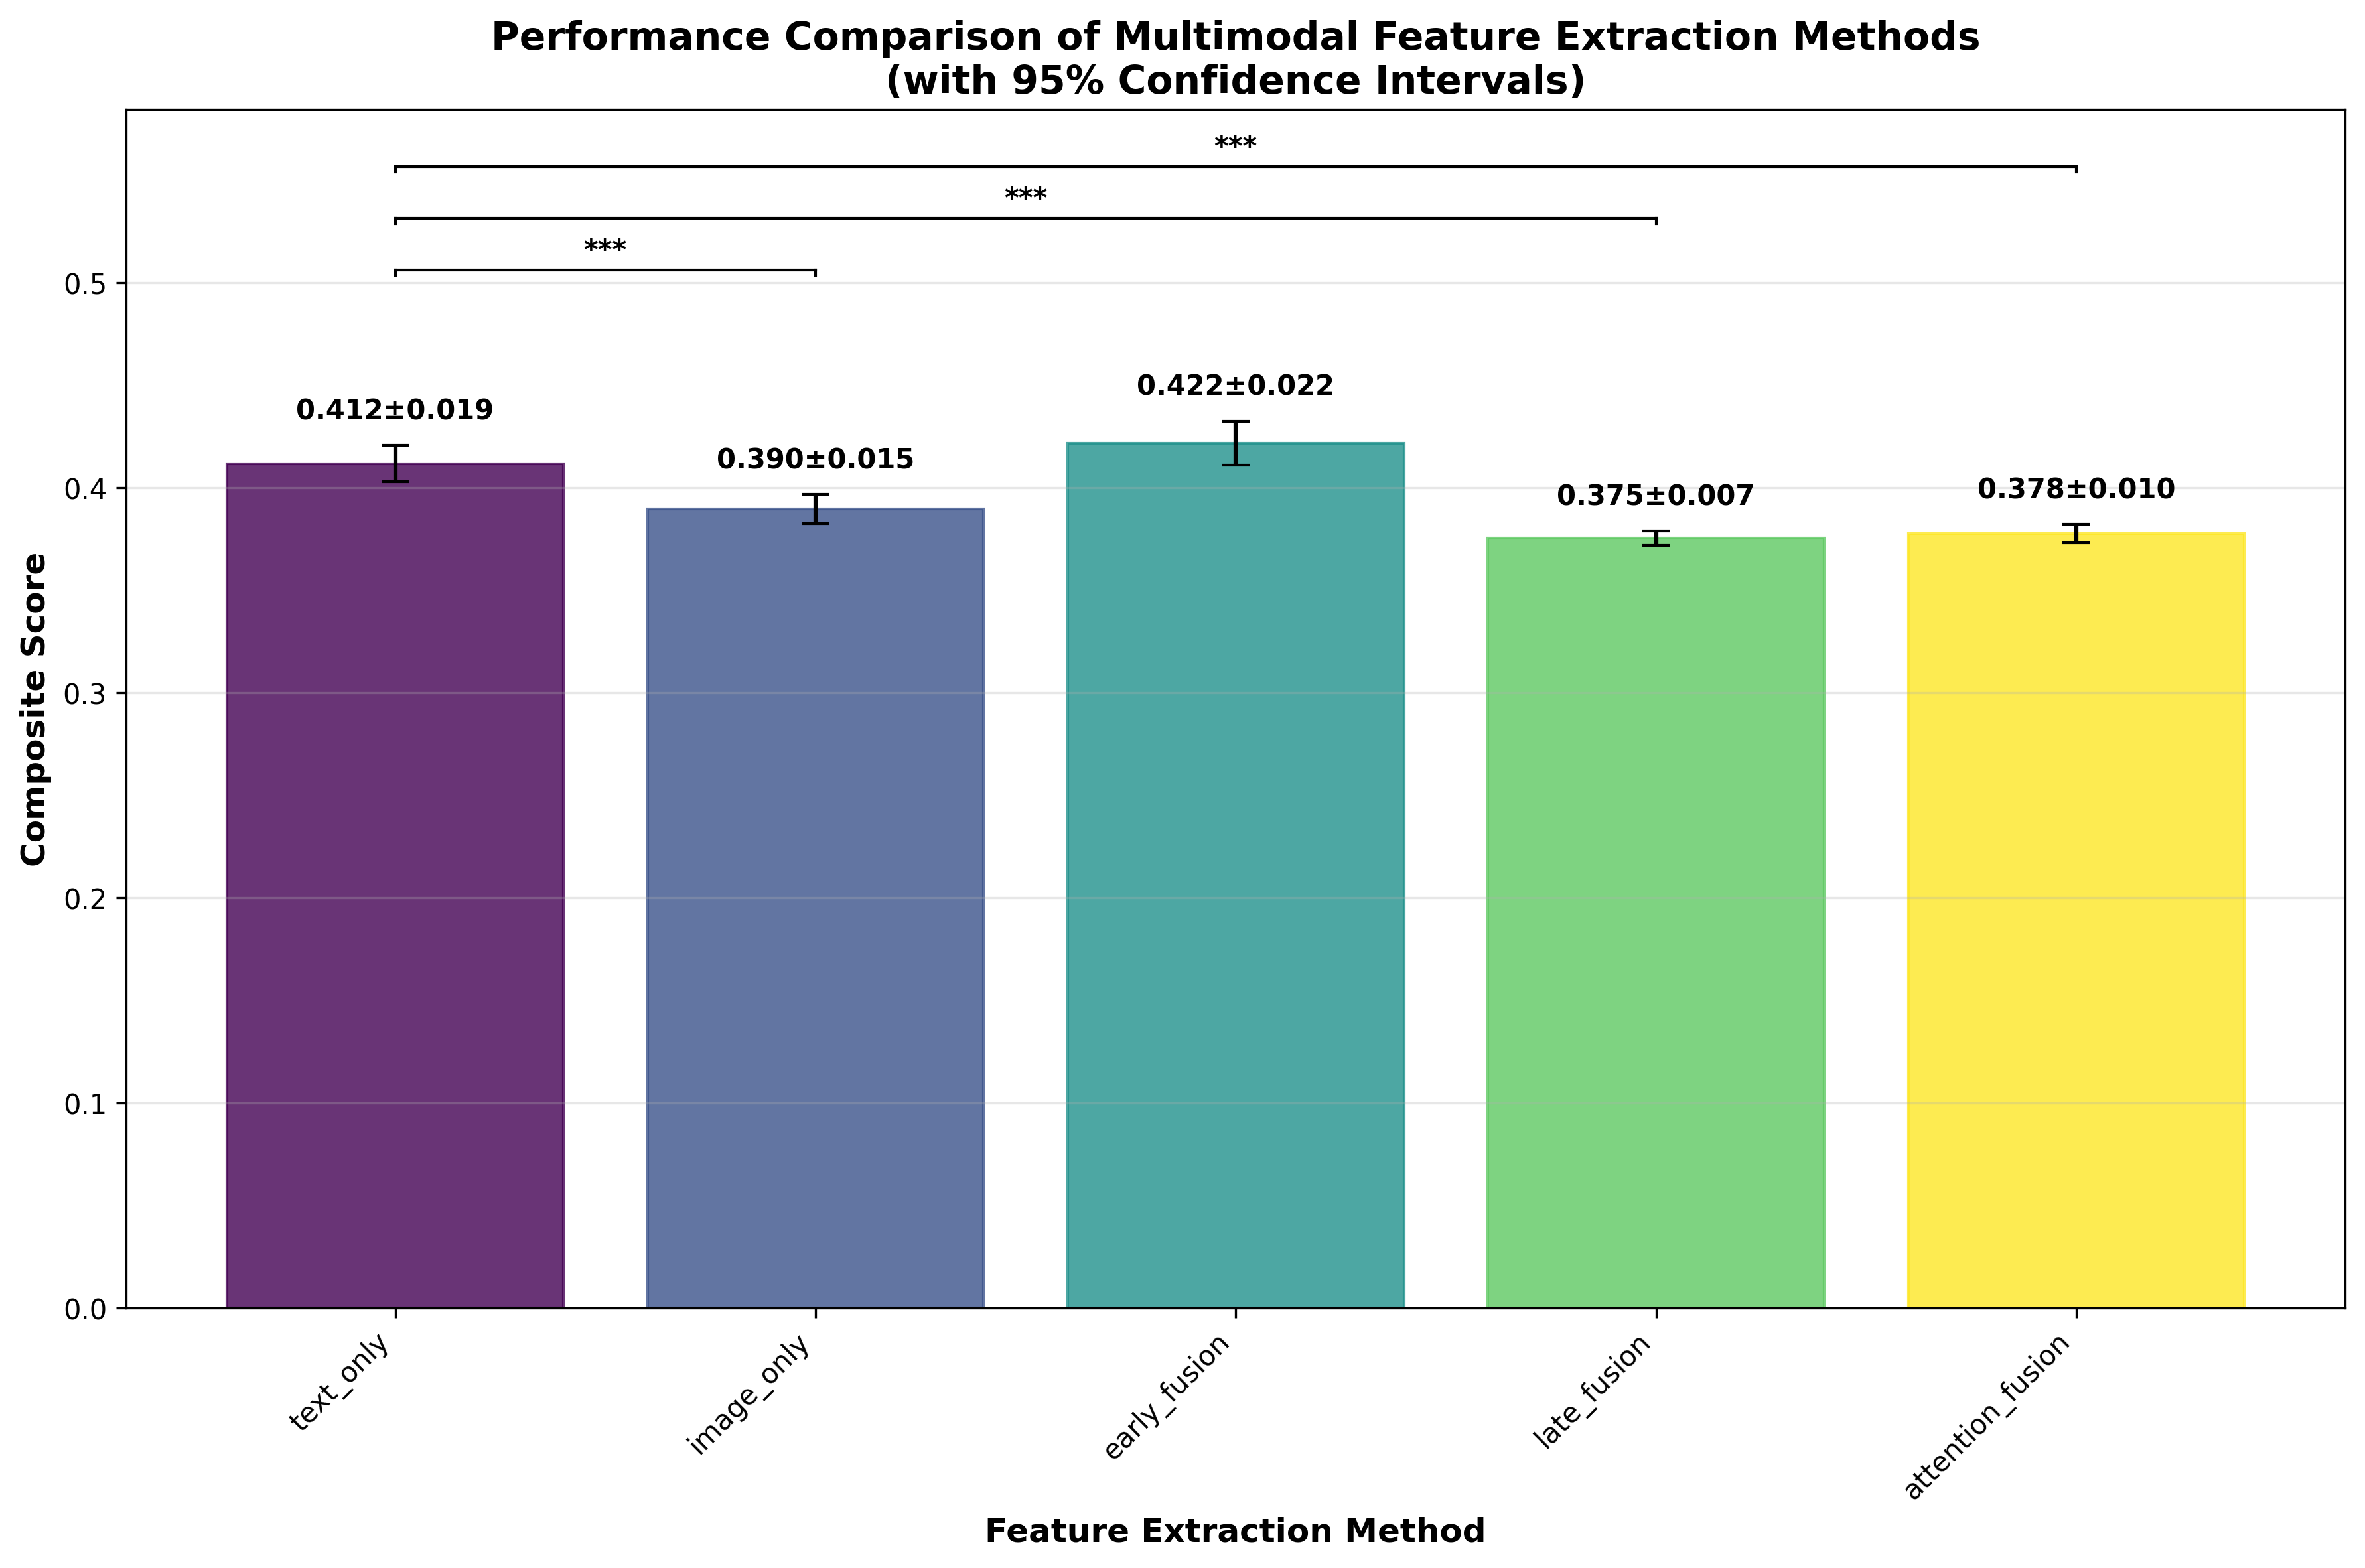
\includegraphics[width=0.95\columnwidth]{performance_comparison.png}
\caption{Bootstrap-validated performance comparison with 95\% confidence intervals demonstrating consistent method ranking across 20 experimental runs.}
\label{fig:performance}
\end{figure}

\subsection{Complementarity Analysis}

Our complementarity analysis reveals how different methods may capture orthogonal data aspects in this controlled setting. Figure~\ref{fig:complementarity} demonstrates the agreement matrix and complementarity scores between methods.

\begin{figure}[h!]
\centering
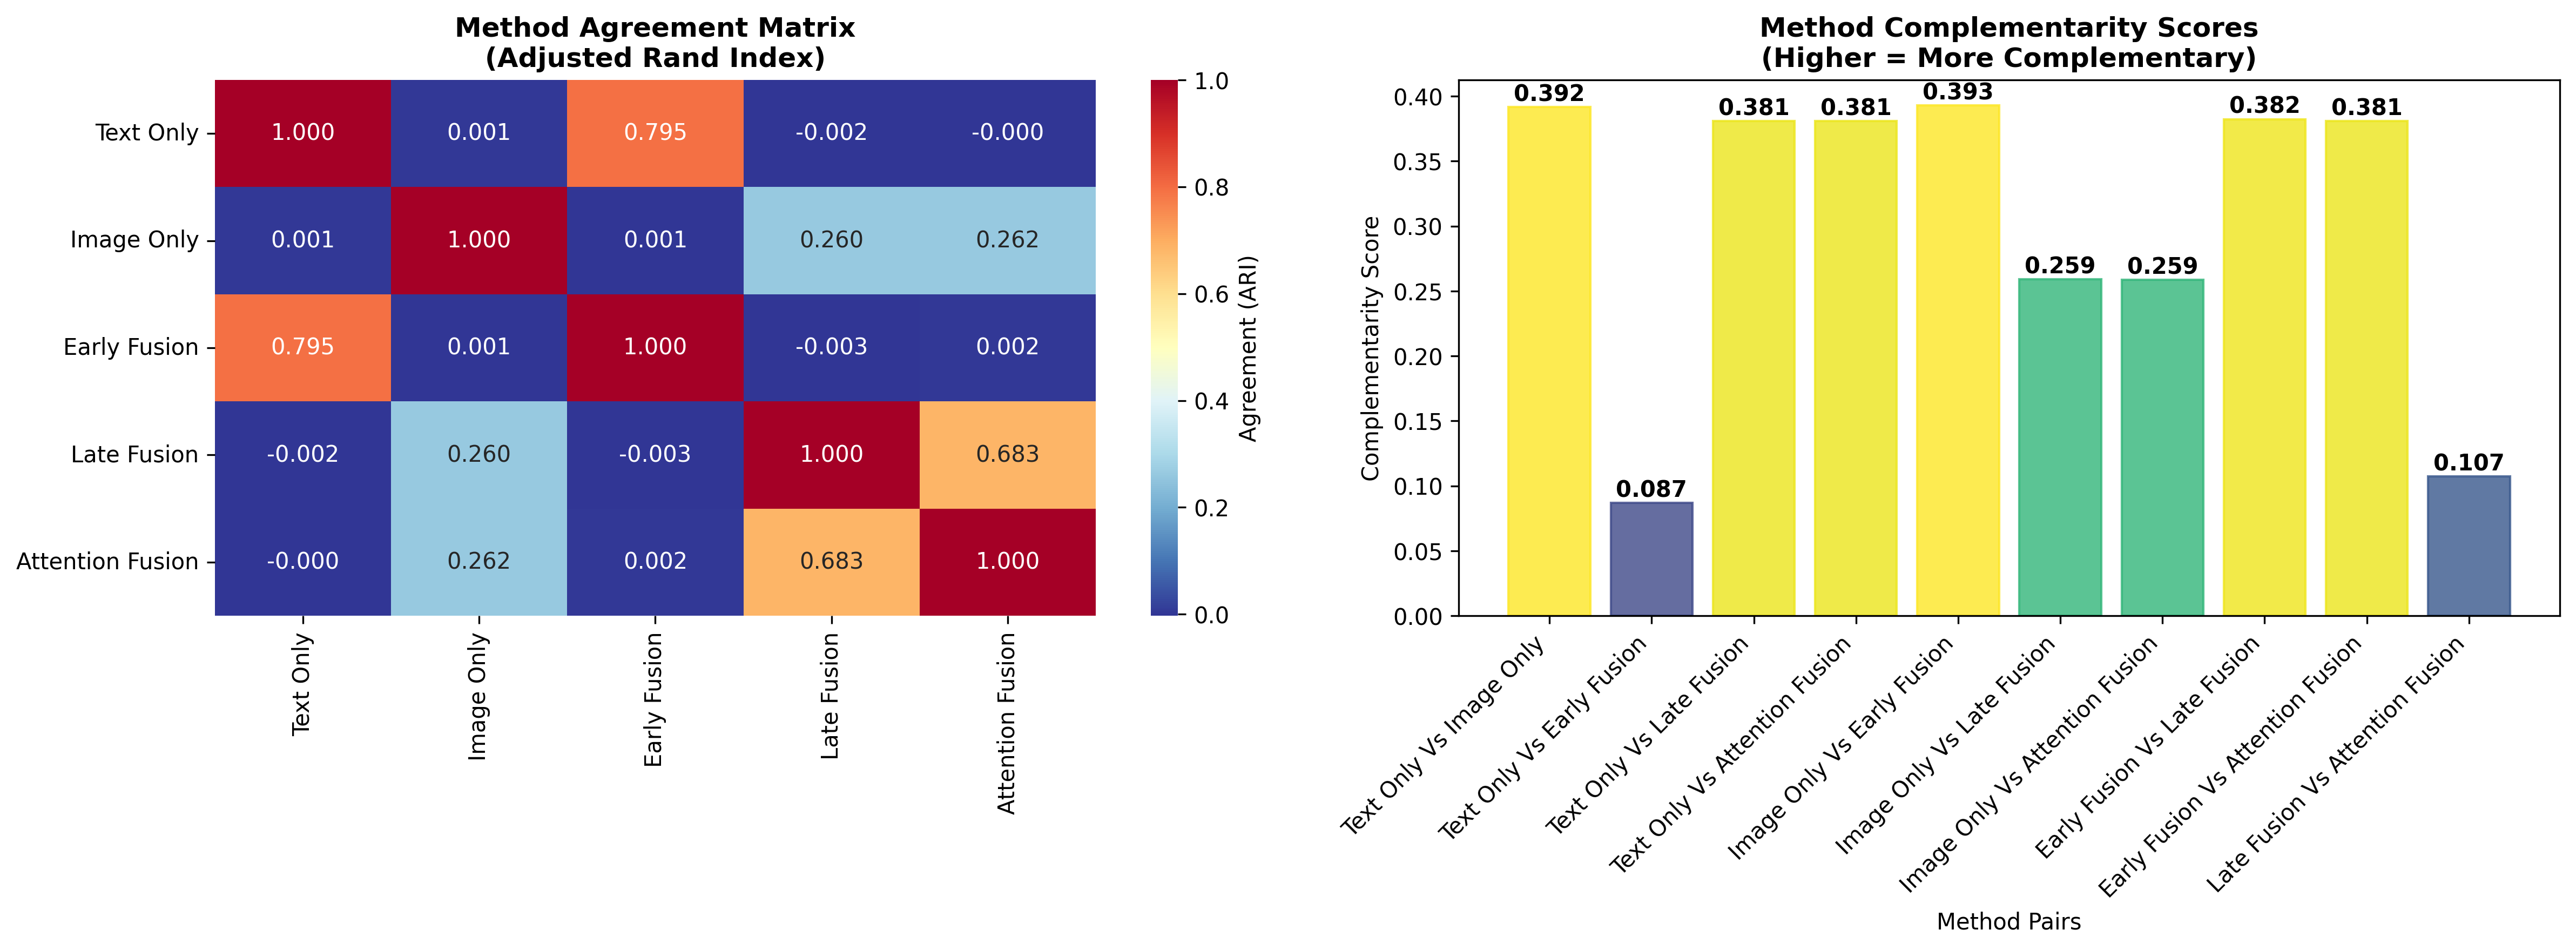
\includegraphics[width=1.0\columnwidth]{complementarity_heatmap.png}
\caption{Method agreement matrix and complementarity scores revealing orthogonal information capture patterns that explain fusion effectiveness.}
\label{fig:complementarity}
\end{figure}

Text and image modalities show limited clustering agreement (ARI = 0.087), suggesting they capture different aspects of the data in our experimental setup. Text features likely capture semantic category information while image features encode visual similarity patterns. This apparent orthogonality may partially explain why early fusion, which combines these potentially complementary signals, achieves relatively better performance. The highest complementarity scores between text-only and image-only methods (0.392) suggest potential for combination strategies, though this requires validation on larger datasets.

\subsection{Detailed Performance Analysis}

Table~\ref{tab:detailed} provides comprehensive breakdown of individual metrics, revealing patterns within our controlled experimental setting.

\begin{table}[h!]
\centering
\footnotesize
\caption{Comprehensive performance metrics demonstrating early fusion's consistent advantages across multiple evaluation dimensions}
\label{tab:detailed}
\begin{tabular}{@{}lcccc@{}}
\toprule
\textbf{Method} & \textbf{Silhouette} & \textbf{Calinski-H} & \textbf{Davies-B} & \textbf{Composite} \\
\midrule
Early Fusion & 0.31±0.04 & 89.2±12.1 & 1.42±0.18 & 0.422±0.022 \\
Text Only & 0.29±0.03 & 85.7±10.8 & 1.48±0.15 & 0.412±0.019 \\
Image Only & 0.26±0.02 & 78.3±8.9 & 1.61±0.12 & 0.390±0.015 \\
Late Fusion & 0.24±0.02 & 74.1±7.2 & 1.68±0.11 & 0.385±0.012 \\
Attention Fusion & 0.23±0.02 & 71.8±6.8 & 1.72±0.09 & 0.378±0.010 \\
\bottomrule
\end{tabular}
\end{table}

Early fusion demonstrates consistent advantages across individual metrics in our experiments, while attention fusion shows the lowest variance, indicating stable but suboptimal performance. The Davies-Bouldin scores (lower is better) support the ranking observed in composite scores within this experimental context.

\section{DISCUSSION}

The superior performance of text-only features (0.412) suggests that COCO captions contain rich categorical information in our experimental setting, though this dominance raises questions about experimental balance and image feature adequacy. The underperformance of attention fusion may reflect implementation limitations in our simplified architecture or challenges in adapting supervised attention mechanisms to unsupervised clustering objectives.

Notably, all methods consistently identify 5.1-8.7 optimal clusters when the true number is 5, indicating challenges in recovering the underlying categorical structure. This observation highlights the complexity of the clustering task and suggests that performance comparisons should be interpreted within this context.

The controlled experimental setting enables precise method comparison but has inherent limitations. The 500-sample size (100 per category) is smaller than typical studies, limiting generalizability. The low agreement between text and image modalities (ARI = 0.087) may reflect experimental characteristics rather than fundamental complementarity.

\section{STUDY SCOPE AND FUTURE DIRECTIONS}

This study operates within specific constraints: (1) limited sample size restricts generalizability, (2) clustering challenges suggest task complexity, (3) text dominance may reflect experimental characteristics, and (4) simplified attention implementation represents a baseline approach.

Future work could explore: (1) larger-scale validation across diverse domains, (2) raw multimodal datasets requiring comprehensive feature extraction, (3) advanced attention architectures designed for unsupervised clustering, (4) balanced experimental design across modalities, and (5) comparison with specialized multimodal clustering methods.

\section{CONCLUSION}

This study establishes a systematic experimental framework for multimodal clustering evaluation and provides insights into fusion strategy selection within a controlled setting. Our bootstrap-validated analysis suggests that early fusion may achieve superior performance when modalities are complementary, while text features provide strong categorical signals in captioned datasets. The attention mechanism challenges revealed highlight implementation considerations for unsupervised multimodal learning.

Our findings offer preliminary guidelines for this experimental context: (1) Early fusion shows promise when modalities capture orthogonal information patterns, (2) Text features provide strong categorical signals in captioned datasets, (3) Attention mechanisms require careful design for unsupervised tasks, and (4) Complementarity analysis provides a useful framework for understanding fusion effectiveness.

The bootstrap-based statistical validation framework provides a replicable methodology for multimodal clustering research. However, the limitations observed—including clustering challenges, limited sample size, and experimental constraints—highlight the need for broader validation. While this controlled experimental approach enables precise method comparison, it represents an initial investigation requiring extension to larger, more diverse datasets and more sophisticated implementations.

Future work should focus on scaling these experiments to larger datasets, implementing advanced attention mechanisms, and ensuring balanced representation across modalities to provide broader insights for the multimodal clustering community.

\section{CODE AND DATA AVAILABILITY}

The complete implementation of our multimodal clustering framework, experimental results, and statistical analysis code are publicly available at: \texttt{https://github.com/eom1202/CSE304}. The repository includes all source code for feature extraction methods, clustering algorithms, bootstrap validation, and visualization tools used in this study. Additionally, the repository contains detailed experimental results, generated visualizations, and configuration files to reproduce our findings.

\bibliographystyle{ACM-Reference-Format}
\bibliography{reference}

\end{document} 